\chapter{Επισκόπηση της Ερευνητικής Περιοχής}
\label{chapter:sota}
Τόσο η αναγνώριση αντικειμένων (object recognition) όσο και η εντοπισμός
της θέσης των αντικειμένων αυτών (detection/localization) σε εικόνες λήψης
είναι μία ερευνητική περιοχή με τεράστιο ενδιαφέρον και
η οποία απασχολεί πληθώρα ερευνητών. Η επιστήμη της Μηχανικής Όρασης (Computer Vision - ML),
στοχεύει στο να δώσει λύσεις στα συγκεκριμένα προβλήματα, εισάγοντας μαθηματικά
μοντέλα, τόσο αναλυτικά, όσο και πιθανοτικά.

O κλάδος της Βαθιάς Μηχανικής Mάθησης (Deep Learning - DL) \cite{Goodfellow-et-al-2016-Book},
ανάγει το πρόβλημα της έυρεσης χαρακτηριστικών σημείων, για την αναγνώριση αντικειμένων,
στην εκμάθηση αναπαραστάσεων \cite{bengio2013representation},
με την χρήση Νευρωνικών Δικτύων Συνέλιξης (Convolutional Neural Networks - CNN).
Οι πρώτες εφαρμογές Νευρωνικών Δικτύων Συνέλιξης, για την αναγνώριση αντικειμένων
σε εικόνες, αναπτύχθηκαν το 1990 από τον Yann LeCun.
Η πιο γνωστή και επιτυχής είναι το δίκτυο LeNet \cite{lecun1998gradient}, το οποίο
χρησιμοποιήθηκε για την αναγνώριση ψηφίων σε εικόνες.
Ωστόσο, η εισαγωγή των CNN στον κλάδο της Μηχανικής Όρασης έγινε το 2012 με
την ανάπτυξη του δικτύου AlexNet \cite{NIPS2012_4824}, από τους Alex Krizhevsky,
Ilya Sutskever και Geoffrey E. Hinton. To δίκτυο AlexNet χρησιμοποιήθηκε
στον διαγωνισμό ImageNet ILSVRC challenge, το 2012, κερδίζοντας με διαφορά
10,9\%, στο σφάλμα αναγνώρισης αντικειμένων σε σύνολο 1000 κλάσεων.
Με την εμφάνιση του δικτύου AlexNet, η ερευνητική κοινότητα ξεκίνησε να
πιστεύει στην αποτελεσματικότητα των Νευρωνικών Δικτύων Συνέλιξης σε εφαρμογές αναγνώρισης
αντικειμένων σε εικόνες. Συνέχεια στο έργο του Alex Krizhevsky έδωσαν οι
ερευνητές αναπτύσσοντας, το 2013, το ZF-Net \cite{DBLP:journals/corr/ZeilerF13}, το οποίο είναι
βασισμένο στην αρχιτεκτονική του δικτύου AlexNet. Μέχρι σήμερα, έχουν σχεδιαστεί
και αναπτυχθεί διάφορα μοντέλα Νευρωνικών Δικτύων Σενέλιξης για
αναγνώριση αντικειμένων, με πιο πρόσφατο το ResNet \cite{DBLP:journals/corr/HeZRS15},
το οποίο αναπτύχθηκε από τον Kaiming He. Το ResNet (Residual Network) έχει την
ιδιαιτερότητα απουσίας πλήρες συνδεδεμένων επιπέδων και είναι από τα πιο δημοφιλες
μοντέλα που εφαρμόζονται σε πρακτικά προβλήματα αναγνώρισης αντικειμένων σε
εικόνες \cite{DBLP:journals/corr/HeZR016}.

Τα προαναφερθέντα μοντέλα Νευρωνικών Δικτύων Συνέλιξης δίνουν
λύσεις μόνο στο πρόβλημα της αναγνώρισης και όχι
του εντοπισμού της θέσης των αντικειμένων αυτών.
Το 2013, ερευνητές εργαζόμενοι στην Google Inc., σχεδίασαν και υλοποίησαν ένα
μοντέλο Νευρωνικού Δικτύου το οποίο δίνει λύσεις στο πρόβλημα της ταυτόχρονης
αναγνώρισης και εντοπισμού αντικειμένων πάνω σε πλαίσια εικόνων \cite{szegedy2013deep}.
Το μοντέλο αυτό, που φέρει το όνομα DetectorNet, είναι ομαδική εργασία των
Christian Szegedy, Alexander Toshev και Dumitru Erhan. Το μοντέλο αυτό είναι
πιθανοτηκό αφού "προβλέπει" τις οριοθετημένες θέσεις για διάφορες κλάσεις
αντικειμένων στον πλαίσιο μίας εικόνας. Ωστόσο, ένα βασικό μειονέκτημα του DetectorNet
που το κάνει ακατάλληλο για εφαρμογή σε προβλήματα πραγματικού χρόνου, όπως
για παράδειγμα σε ένα ρομποτικό σύστημα, είναι οι τεράστιες απαιτήσεις του σε πόρους
και χρόνο.
\\

\textbf{TODO: A few words about the applications of DNN models in robotics!!!!}

%\section{Deep Neural Networks}
\label{sec:theory_dnn}

The computations involved in producing an output from an input can be represented by a flow graph: a flow graph is a graph representing a computation, in which each node represents an elementary computation and a value (the result of the computation, applied to the values at the children of that node). Consider the set of computations allowed in each node and possible graph structures and this defines a family of functions. Input nodes have no children. Output nodes have no parents.

%\section{Νευρωνικά Δίκτυα Συνέλιξης}
\label{sec:theory_cnn}

Μέχρι τώρα μιλήσαμε για τα πολυεπίπεδα νευρωνικά δίκτυα και την γενικότερη
λειτουργία τους. Σε αυτό το υποκεφάλαιο θα μιλήσουμε για συγκεκριμένα μοντέλα
πολυεπίπεδων νευρωνικών δικτύων και πιο συγκεκριμένα για τα
\emph{νευρωνικά Δίκτυα Συνέλιξης}. Τα συγκεκριμένα μοντέλα χρησιμοποιούνται
σήμερα κυρίως στα προβλήματα της αναγνώρισης και εντοπισμού αντικειμένων
σε εικόνες.

Ο τρόπος λειτουργίας τους είναι όμοιος με αυτόν που παρουσιάστηκε στο
\autoref{sec:dnn}; αποτελούνται από πολλά επίπεδα, όπου το κάθε επίπεδο αποτελείται
από έναν αριθμό νευρώνων οι οποίοι έχουν σαν παραμέτρους εκμάθησης τα βάρη ($w_{\jmath}^{\imath}$) τους
και την τιμή πόλωσης ($b^{\imath}$).
Κάθε νευρώνας δέχεται ένα σήμα εισόδου , εφαρμόζει μία πράξη εσωτερικού γινομένου σε αυτό,
και προαιρετικά περνάει το αποτέλεσμα από μία μη γραμμική συνάρτηση.
Το τελευταίο επίπεδο των CNN είναι ένας πλήρες συνδεδεμένο επίπεδο και έχει μία
συνάρτηση σφάλματος.
Η διαφορά των μοντέλων CNN από τα κλασσικά ANN είναι ότι θεωρούν για δεδομένα εισόδου
εικόνες.

Αυτό που καταφέρνουν να κάνουν τα CNN είναι να μοντελοποιήσουν μικρά
κομμάτια πληροφορίας τα οποία στην συνέχεια ενώνονται για να δημιουργήσουν
υψηλότερου επιπέδου πληροφορία. Αν για παράδειγμα παρατηρήσουμε την λειτουργία
ενός μοντέλου CNN, το πρώτο επίπεδο προσπαθεί να εντοπίσει ακμές, το δεύτερο
επίπεδο και παίρνοντας την πληροφορία αυτή των ακμών προσπαθεί να εντοπίσει περιγράμματα,
κτλ.


Σε κάθε πίξελ της εικόνας αντιστοιχούν 3 τιμές (RGB) και άρα η είσοδος σε ένα
CNN έχει τρεις διαστάσεις όπως φαίνεται και στο \autoref{fig:cnn_1}.
Για παράδειγμα ένα CNN το οποίο έχει σχεδιαστεί να δέχεται σαν είσοδο εικόνες ανάλυσης $80\times60$
έχει επίπεδο εισόδου διαστάσεων $80\times60\times3$.

\begin{figure}[!ht]
  \centering
  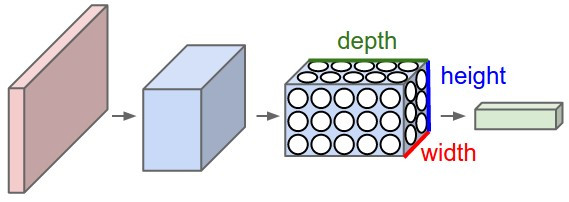
\includegraphics[width=0.8\textwidth]{./images/chapter3/cnn.jpg}
  \caption[Τρισδιάστατη κατανομή των νευρώνων στα CNN]{Τρισδιάστατη κατανομή των νευρώνων στα CNN}
  \label{fig:cnn_1}
\end{figure}

Κάθε επίπεδο ενός CNN παίρνει σαν είσοδο μία μορφή όγκου την οποία
και μετασχηματίζει σε μία άλλη μορφή όγκου.

Οι τρεις βασικοί τύποι επιπέδων που χρησιμοποιούνται σε αρχιτεκτονικές CNN είναι:
\begin{itemize}
  \item{Επίπεδο Συνέλιξης - Convolutional Layer (CONV)}
  \item{Επίπεδο Υπό-δειγματοληψίας- Pooling Layer (POOL)}
  \item{Πλήρη Συνδεδεμένο Επίπεδο - Fully-Connected Layer (FC)}
\end{itemize}
Μία σημαντική παρατήρηση είναι ότι τα επίπεδα CONV και FC έχουν παραμέτρους, δηλαδή
βάρη και τιμή πόλωσης των νευρώνων, ενώ τα επίπεδα POOL εκτελούν λειτουργία
δειγματοληψίας στα δεδομένα εισόδου τους.


\subsection{Επίπεδο Συνέλιξης}

Τα επίπεδα συνέλιξης είναι ο πυρήνας των μοντέλων CNN. Οι παράμετροι ενός
επιπέδου CONV είναι μία σειρά από δισδιάστατα φίλτρα τα οποία όμως εκτείνονται
σε όλο το σε όλο το βάθος του όγκου εισόδου. Το βάθος των φίλτρων αυτών
ισούται με το βάθος του όγκου στην είσοδο.


Όπως αναφέραμε και προηγουμένως, τα επίπεδα CONV εφαρμόζουν πράξη συνέλιξης πάνω στα
δεδομένα εισόδου. Αυτό επηρεάζει στην δομή των "τοπικών" διασυνδέσεων.
Στο παράδειγμα του σχήματος \ref{fig:cnn_2} βλέπουμε πως ο κάθε νευρώνας
του επιπέδου συνέλιξης συνδέεται με μία περιοχή του όγκου στην είσοδό του.

\begin{figure}[!ht]
  \centering
  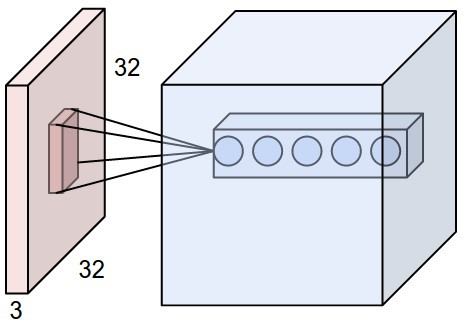
\includegraphics[width=0.4\textwidth]{./images/chapter3/cnn_2.jpg}
  \caption[%
    Παράδειγμα διασύνδεσης τρισδιάστατης εισόδου με την τρισδιάστατη δομή των
    νευρόνων ενός επιπέδου συνέλιξης (CONV)]{%
    Παράδειγμα διασύνδεσης τρισδιάστατης εισόδου με την τρισδιάστατη δομή των
    νευρόνων ενός επιπέδου συνέλιξης (CONV)}
  \label{fig:cnn_2}
\end{figure}

Η συνέλιξη ενός φίλτρου με τον τον όγκο εισόδου παράγει έναν \emph{χάρτη ενεργοποίησης (activation map)},
με τον τρόπο που φαίνεται στο \autoref{fig:cnn_activation_map}. Στο παράδειγμα αυτό
εφαρμόζεται φίλτρο διαστάσεων $5\times5\times3$ σε έναν όγκο $32\times32\times3$ και παράγεται
ένας χάρτης ενεργοποίησης διαστάσεων $28\times28\times1$.

\begin{figure}[!ht]
  \centering
  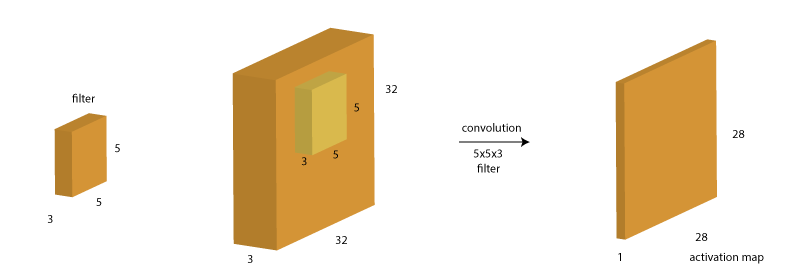
\includegraphics[width=1\textwidth]{./images/chapter3/cnn_activation_map.png}
  \caption[Συνέλιξη φίλτρου ενός επιπέδου συνέλιξης με τον όγκο εισόδου και παραγωγή ενός χάρτη ενεργοποίησης]{Συνέλιξη φίλτρου ενός επιπέδου συνέλιξης με τον όγκο εισόδου και παραγωγή ενός χάρτη ενεργοποίησης}
  \label{fig:cnn_activation_map}
\end{figure}

Η μείωση των διαστάσεων μήκους και πλάτους από $32\times32$ σε $28\times28$ οφείλεται στον τρόπο με τον οποίο
εκτελείται η πράξη της συνέλιξης των φίλτρων με τον όγκο εισόδου  (\autoref{fig:cnn_conv}).
Οι διαστάσεις του όγκου εξόδου, έχοντας σαν είσοδο όγκο διαστάσεων $N \times N \times d$ και φίλτρων $F \times F \times d$ υπολογίζονται, στην απλούστερη περίπτωση με βάση την σχέση
\begin{equation*}
  outsize = (N-F) + 1
\end{equation*}


\begin{figure}[!ht]
  \centering
  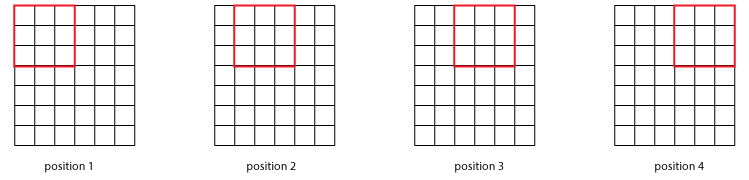
\includegraphics[width=1\textwidth]{./images/chapter3/cnn_conv.png}
  \caption[Διαδικασία Συνέλιξης]{Διαδικασία Συνέλιξης}
  \label{fig:cnn_conv}
\end{figure}

Η τιμή του βάθους του όγκου στην έξοδο ενός επιπέδου CONV αντιστοιχεί στον αριθμό των φίλτρων που
εφαρμόζονται στον όγκο εισόδου. Δηλαδή ο αριθμός των χαρτών ενεργοποίησης
αντιστοιχεί στον αριθμό των φίλτρων. Αν για παράδειγμα ο όγκος εισόδου είναι
διαστάσεων $32\times\32\times3$ και εφαρμόσουμε δέκα φίλτρα συνέλιξης διαστάσεων $5\times5\times3$,
ο όγκος εξόδου θα είναι διαστάσεων $28\times28\times3$ \autoref{fig:cnn_num_filters}.
Ο αριθμός των φίλτρων είναι μία παράμετρος, ή καλύτερα \emph{υπερ-παράμετρος} των επιπέδων συνέλιξης.

\begin{figure}[!ht]
  \centering
  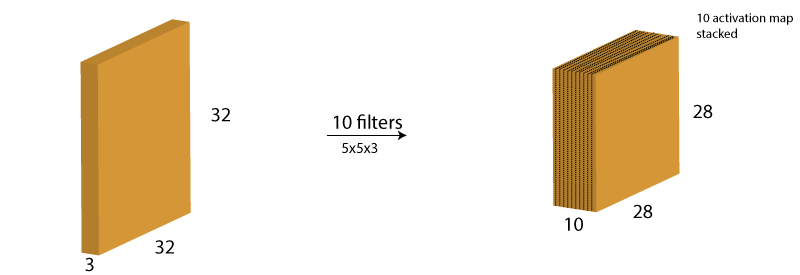
\includegraphics[width=1\textwidth]{./images/chapter3/cnn_num_filters.png}
  \caption[Αντιστοιχία του αριθμού των φίλτρων ενός επιπέδου συνέλιξης με το βάθος του όγκου στην έξοδο]{Αντιστοιχία του αριθμού των φίλτρων ενός επιπέδου συνέλιξης με το βάθος του όγκου στην έξοδο}
  \label{fig:cnn_num_filters}
\end{figure}

Ωστόσο, το βήμα μετατόπισης (stride) του φίλτρου πάνω στην είσοδο είναι και αυτό
μία υπέρ-παράμετρος (hyperparameter) των επιπέδων συνέλιξης.
Χρησιμοποιώντας βήμα μετατόπισης (S) διάφορο της μονάδας καταλήγουμε στην πιο κάτω
εξίσωση για τον υπολογισμό του όγκου εξόδου:
\begin{equation*}
  outsize = (N-F)/S + 1
\end{equation*}

Ένα πρόβλημα που εμφανίζεται στην περίπτωση των μοντέλων CNN με μεγάλο αριθμό
κρυφών επιπέδων είναι η γρήγορη μείωση των διαστάσεων μήκους και πλάτους του
όγκου, το οποίο είναι αποτέλεσμα της διαδοχική εφαρμογή πράξεων συνέλιξης (\autoref{fig:cnn_shrunk}).

\begin{figure}[!ht]
  \centering
  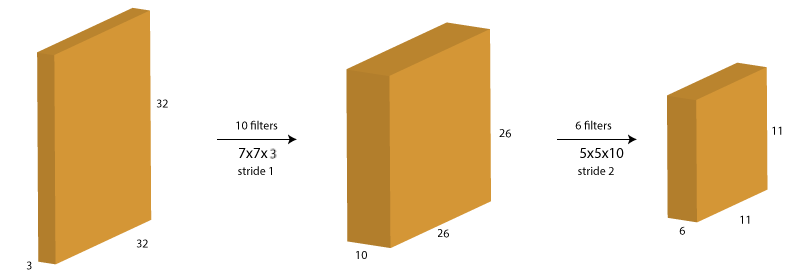
\includegraphics[width=1\textwidth]{./images/chapter3/cnn_shrunk.png}
  \caption[Διαδοχικές εφαρμογές του τελεστή συνέλιξης προκαλούν μείωση των διαστάσεων μήκους και πλάτους του όγκου]{Διαδοχικές εφαρμογές του τελεστή συνέλιξης προκαλούν μείωση των διαστάσεων μήκους και πλάτους του όγκου}
  \label{fig:cnn_shrunk}
\end{figure}

Αυτή η συμπεριφορά είναι ανεπιθύμητη αφού περιορίζει και τις διαστάσεις των φίλτρων
που μπορούμε να χρησιμοποιήσουμε σε κάθε επίπεδο CONV. Η χρήση φίλτρων μεγάλων
διαστάσεων φέρει σαν αποτέλεσμα την γρήγορη μείωση των διαστάσεων του όγκου.

Για να αποτρέψουμε αυτή την συμπεριφορά μπορούμε να επεκτείνουμε τις διαστάσεις
μήκους και πλάτους, προσθέτοντας μηδενικά στα σύνορα του όγκου εισόδου του
εκάστοτε επιπέδου CONV. Η διαδικασία αυτή ονομάζεται
\emph{zero-padding} και φαίνεται στο \autoref{fig:cnn_zero_padding}.
\begin{figure}[!ht]
  \centering
  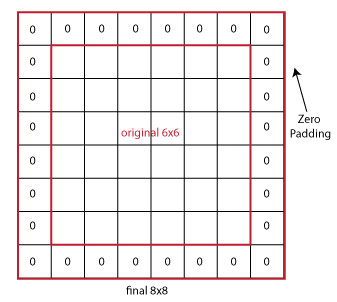
\includegraphics[width=0.6\textwidth]{./images/chapter3/cnn_zero_padding.png}
  \caption[Zero Padding]{Zero Padding}
  \label{fig:cnn_zero_padding}
\end{figure}
Το μέγεθος του συνόρου που προστίθεται είναι η τρίτη υπέρ-παράμετρος ενός
επιπέδου συνέλιξης.

Με την εισαγωγή της υπέρ-παραμέτρου zero-padding η εξίσωση υπολογισμού του όγκου
εξόδου έχει την μορφή:
\begin{equation*}
  outsize = (N - F + 2P)/S + 1
\end{equation*}

Συνοψίζοντας, ένα επίπεδο συνέλιξης έχει τα εξής χαρακτηριστικά:
\begin{itemize}
  \item{Διαστάσεις όγκου εισόδου: $W_{1} \times H_{1} \times D_{1}$}
  \item{Hyperparameters:}
    \begin{itemize}
      \item{K: Αριθμός φίλτρων}
      \item{F: Μέγεθος του φίλτρου ($F \times F$)}
      \item{S: Βήμα μετατόπισης}
      \item{P: Ποσότητα zero-padding}
    \end{itemize}
  \item{Διαστάσεις όγκου εξόδου: $W_{2} \times H_{2} \times D_{2}$, $D_{2} = K$} όπου:
    \begin{itemize}
      \item{$W_{2} = (W_{1} - F)/S + 1$}
      \item{$H_{2} = (H_{1} - F)/S + 1$}
      \item{$D_{2} = D_{1}$}
    \end{itemize}
\end{itemize}


\subsection{Επίπεδο Υπό-δειγματοληψίας - Pooling layer}

Συνήθως τα επίπεδα υπό-δειγματοληψίας προστίθενται στο δίκτυο, μεταξύ διαδοχικών
επιπέδων συνέλιξης. Η λειτουργία τους είναι να μειώσουν τις χωρικές
διαστάσεις των αναπαραστάσεων, μειώνοντας έτσι τον αριθμό των
παραμέτρων και άρα τους υπολογισμούς που γίνονται στο νευρωνικό δίκτυο
(\autoref{fig:cnn_pool}).

\begin{figure}[!ht]
  \centering
  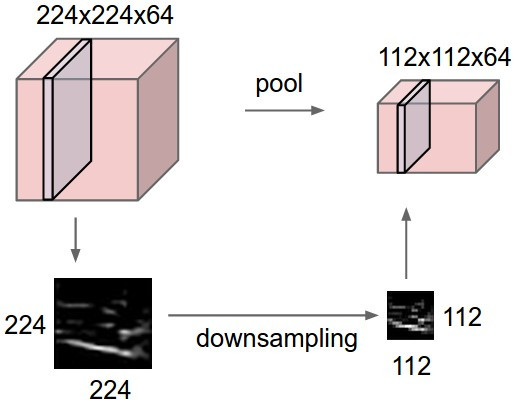
\includegraphics[width=0.6\textwidth]{./images/chapter3/cnn_pool.jpg}
  \caption[Επίπεδο Υποδειγματοληψίας - Pooling layer]{Επίπεδο Υπό-δειγματοληψίας - Pooling layer}
  \label{fig:cnn_pool}
\end{figure}
Ενεργεί δηλαδή σαν μία συνάρτηση υπό-δειγματοληψίας.
Πιθανές συναρτήσεις υπό-δειγματοληψίας είναι οι συναρτήσεις \emph{max, average και L2-Norm}

Στο \autoref{fig:cnn_pool_max} βλέπουμε το αποτέλεσμα της εφαρμογή της συνάρτησης
δειγματοληψίας $max(\vec{v})$ πάνω σε ένα πλέγμα διαστάσεων $4 \times 4$.

\begin{figure}[!ht]
  \centering
  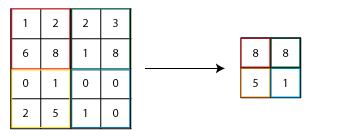
\includegraphics[width=0.6\textwidth]{./images/chapter3/cnn_pool_max.png}
  \caption[Συνάρτηση υπό-δειγματοληψίας Max - Max Pooling]{Συνάρτησης υποδειγματοληψίας Max - Max Pooling}
  \label{fig:cnn_pool_max}
\end{figure}

Τα χαρακτηριστικά των συναρτήσεων υπό-δειγματοληψίας είναι:
\begin{itemize}
  \item{Διαστάσεις όγκου εισόδου: $W_{1} \times H_{1} \times D_{1}$}
  \item{Hyperparameters:}
    \begin{itemize}
      \item{F: Χωρική τους έκταση ($F \times F$)}
      \item{S: Βήμα μετατόπισης}
    \end{itemize}
  \item{Διαστάσεις όγκου εξόδου: $W_{2} \times H_{2} \times D_{2}$, $D_{2} = K$} όπου:
    \begin{itemize}
      \item{$W_{2} = (W_{1} - F)/S + 1$}
      \item{$H_{2} = (H_{1} - F)/S + 1$}
      \item{$D_{2} = D_{1}$}
    \end{itemize}
\end{itemize}


\subsection{Πλήρως Συνδεδεμένο Επίπεδο - Fully-connected layer}

Ένα πλήρως συνδεδεμένο επίπεδο συνδέεται με όλους τους νευρώνες στο
προηγούμενο επίπεδο, όπως γίνεται στα απλά μοντέλα NN (Πολυεπίπεδος Perceptron),

Συνήθως το τελευταίο επίπεδο σε ένα CNN είναι πλήρως συνδεδεμένο και πιο
συγκεκριμένα έχει τόσους νευρώνες όσες και οι κλάσεις της πρόβλεψης. Για
παράδειγμα, ένα CNN που χρησιμοποιείται για αναγνώριση αντικειμένων σε
εικόνες CIFAR-10 έχει το τελευταίο επίπεδο του πλήρως συνδεδεμένο και
αποτελείται από 10 νευρώνες.

